\section{Localization and Object Detection}
\subsection{Localization}
The input image contains a single relevant object to be classified in a fixed set of categories. The task is:
\begin{itemize}
    \item Assign the object class to the image
    \item Locate the object in the image by its bounding box
\end{itemize}{}

The task is a prediction task which involve a discrete output and 4 different outputs which are the bounding box limits. 

\subsubsection{Simplest Solution}
The network have to be both a \textit{classification} network and a \textit{regression} network to identify bounding boxes, so you need to combine two different losses. The training loss has to be a single scalar since we compute gradient of a scalar function w.r.t. network parameters. The idea is to minimize a multitask loss to merge two losses:
$$
\mathcal{L}(x)=\alpha \delta(x)+(1-\alpha) \mathcal{R}(x)
$$
where the hyper-parameter $\alpha$ is used to balance the losses to make the two losses in a similar range. Watch out that $\alpha$ directly influences the loss definition, so tuning might be difficult, better to do cross-validation looking at some other loss.\\
So you will have \textit{two different ends} of your network, one part with $L$ (number of classes) neurons, and the other will predict the 4 bounding boxes. \\ \\
Human-Pose Estimation is formulated as a \textbf{CNN-regression problem} towards \textit{body joints}. The network receives as input the whole image, capturing the full-context of each body joints.
The approach is very simple to design and train. Training problems can be alleviated by transfer learning of existing classification networks. 
Pose is defined as a vector of $k$ joints location for the human body, possibly normalized w.r.t. the bounding box enclosing the human. 

\subsubsection{Weakly-Supervised Localization}
Perform localization over an image without any annotating bounding box. So you train your network as a classification network to assign to each image a label, but you want also your network to perform localization. The only form of supervision is the classification label, not the bounding box: only the classification labels are provided.\\ \\
This is a sort of Global Averaging Pooling \textit{revisited}: the advantages of GAP layer extend beyond simply acting as a structural regularizer that prevents overfitting; in fact, the network can retain a remarkable localization ability until the final layer. By a simple tweak it is possible to easily identify the discriminative image regions leading to a prediction.\\
\begin{quote}
    \textit{A CNN trained on \textbf{object categorization} is successfully able to localize the discriminative regions for action classification as the object that the humans are interacting with rather than the humans themselves}
\end{quote} 

Your network takes in input an image and provides a big volume. The larger of image, the larger the volume is. In case of classification, you have to squeeze down this volume to a fixed size, which is the input of the fully connected layer. \\
An option is to \textit{resize} the image, the other option is to introduce another \textit{GAP layer}: average the values of each slice of the volume. So you have a vector with a value for each one of the $n$ slices and, at the end, what you get is a vector of length $n$. \\
\textit{GAP} is shown to perform better in some cases than Dropout in order to perform Regularization. This is why it is useful, it's \underline{reduce overfitting} and can be used with \underline{images of any shape}. 

\begin{wrapfigure}{l}{6cm}
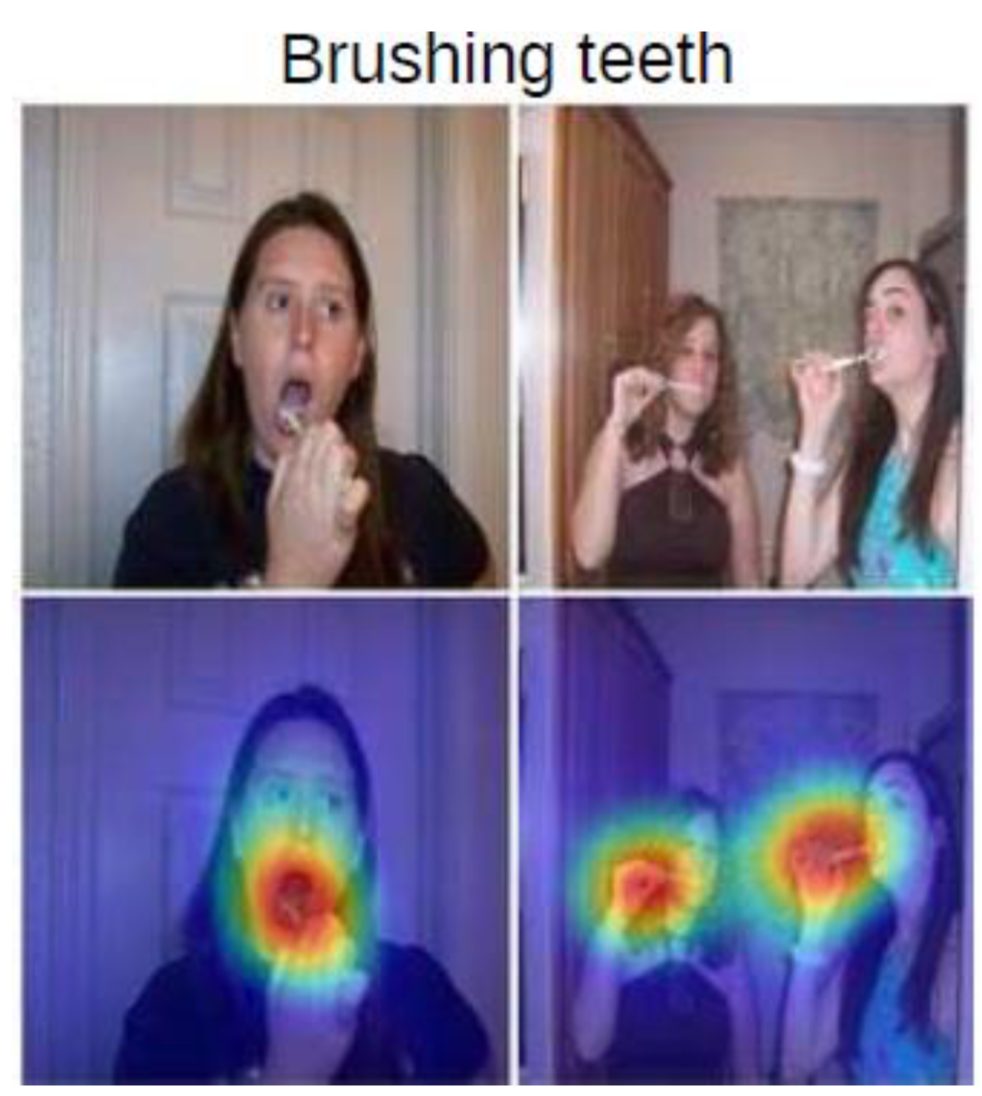
\includegraphics[width=5cm]{images/heatmap_localization.png}
\caption{Heatmaps}\label{wrap-fig:heatmap_loc}
\end{wrapfigure} 

In the paper, GAP it is also presented as a tool to modify slightly your network and get instead a classification network, a network that perform a sort of Localization: it is able to localize discriminative regions for the classification task at the object that human are interactive with. In fact, the heatmaps show which is the image region which has mostly influenced the network decision. This kind of heatmap is perfect to identify bounding boxes. 

The nice part of the story is that if you take any classification network, you introduce a GAP layer, you get for free a network that is able to provide that sort of heatmap, so you are able to perform Localization. \\ \\
This approach of identifying exactly which regions of an image are being used for discrimination is called \textbf{Class Activation Map}: it is very easy to compute since it just requires an FC layer after the GAP and a minor tweak. \\

 \begin{wrapfigure}{r}{7cm}
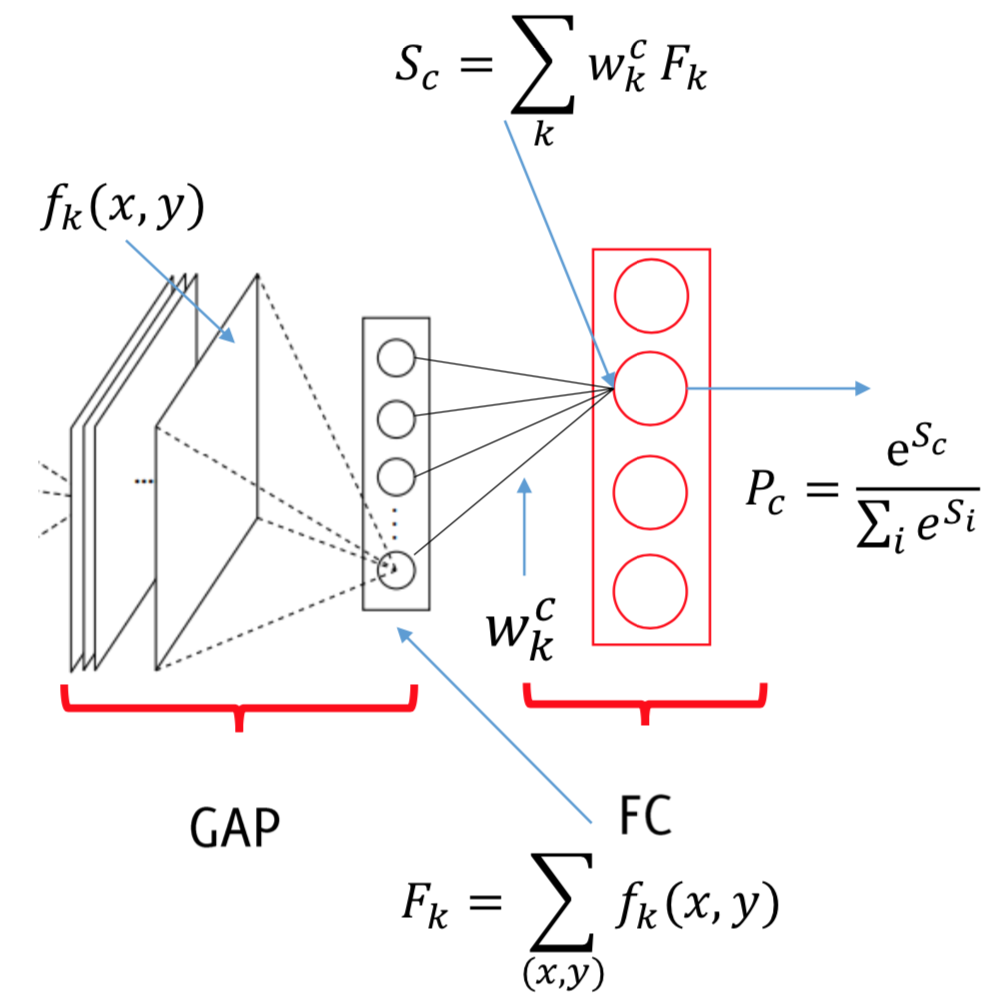
\includegraphics[width=7cm]{images/GAP_layer.png}
\caption{GAP layer}\label{wrap-fig:gap_layer}
\end{wrapfigure} 

Considering Fig.\ref{wrap-fig:gap_layer}, a very simple architecture made only of convolutions and activation functions leads to a final layer having: 
\begin{itemize}
    \item[--] $n$ feature maps $f_k(:,:)$ having resolution "similar" to the input image
    \item[--] a vector after GAP made of $n$ averages $F_k$
\end{itemize}
The FC layer after the GAP it's the output layer which computes $S_c$ for each class $c$ by the weighted sum of {$F_k$}, where weights $w_k^c$ are defined during training. Then, we can extract the class probability $P_c$ via softmax, for each class $c$. The weights $w_k^c$ encodes the importance of $F_k$ for the class $c$ 
$$
S_c = \sum_{k=1}^{N} w_k^{c}F_k = \sum_{k=1}^{N} w_k^{c} \sum_{x,y} f_k(x,y) = \sum_{x,y} \sum_{k} w_k^c f_k(x,y)
$$
\\ \\
%after the last part of convolution of the network, we perform a GAP and we get a vector of size $n$, where $n$ is the number of slices of the last convolutional layer. We call $F_1$ the average of the fist slice, $F_2$ the average of the second layer and so on. Now you can just introduce a simple output layer, so in case of a classifier, you have a fully-connected layers with n neurons. So once you train, you have multiple weights $w_1$, $w_2$ and so on. When you feed an image, you can take the softmax to obtain the predicted class; then you can take the weights: let's call the weights $w_{i}^c$, where c defines the specific class and i the i-th value, and the score is:

So you can construct an image where in each pixel there is the linear combination of all the weights corresponding to a slices rescaled by the corresponding weighth $w_k^c$. The image in the output is exactly the heatmap which highlights which part of the image contributes more on the decision of the network. The results is called Class Activation Map which is defined as:
$$
M_{c}(x, y)=\sum_{k} w_{k}^{c} f_{k}(x, y)
$$
where $M_{c}(x, y)$ directly indicates the importanc of the acrivations at $(x,y)$ for predicting the class $c$. Thanks to the softmax, the depth of the last convolutional volume can differ from the number of classes. 
%linear combination between all the slices * the corresponding weight.

%Important: slide 18: dando in input l'immagine, più passa per la convoluzione, più il blocco di convoluzione diventa piccolo. Per farlo tornare alla grandezza dell'immagine in modo da avere delle heatmap della stessa grandezza dell'immagine di input, dobbiamo fare upsampling. Un'altra opzione sarebbe quella di fare una sorta di U-net come la segmentation, si ottiene più resolution ma less semantic. \\
When we feed the CNN with an input image, we get a convolutional block (the volume) which becomes smaller as the input pass through the network. We need to perform an upsampling to obtain the an heatmap of the same size of the input image. Another option would be to perform a sort of U-net as the segmentation problem, obtaining more resolution but less semantic. \\
As shown in Fig.\ref{fig:cam}, the weights represents the importance of each feature map to yield the final prediction.

 \begin{figure}[h]
    \centering
    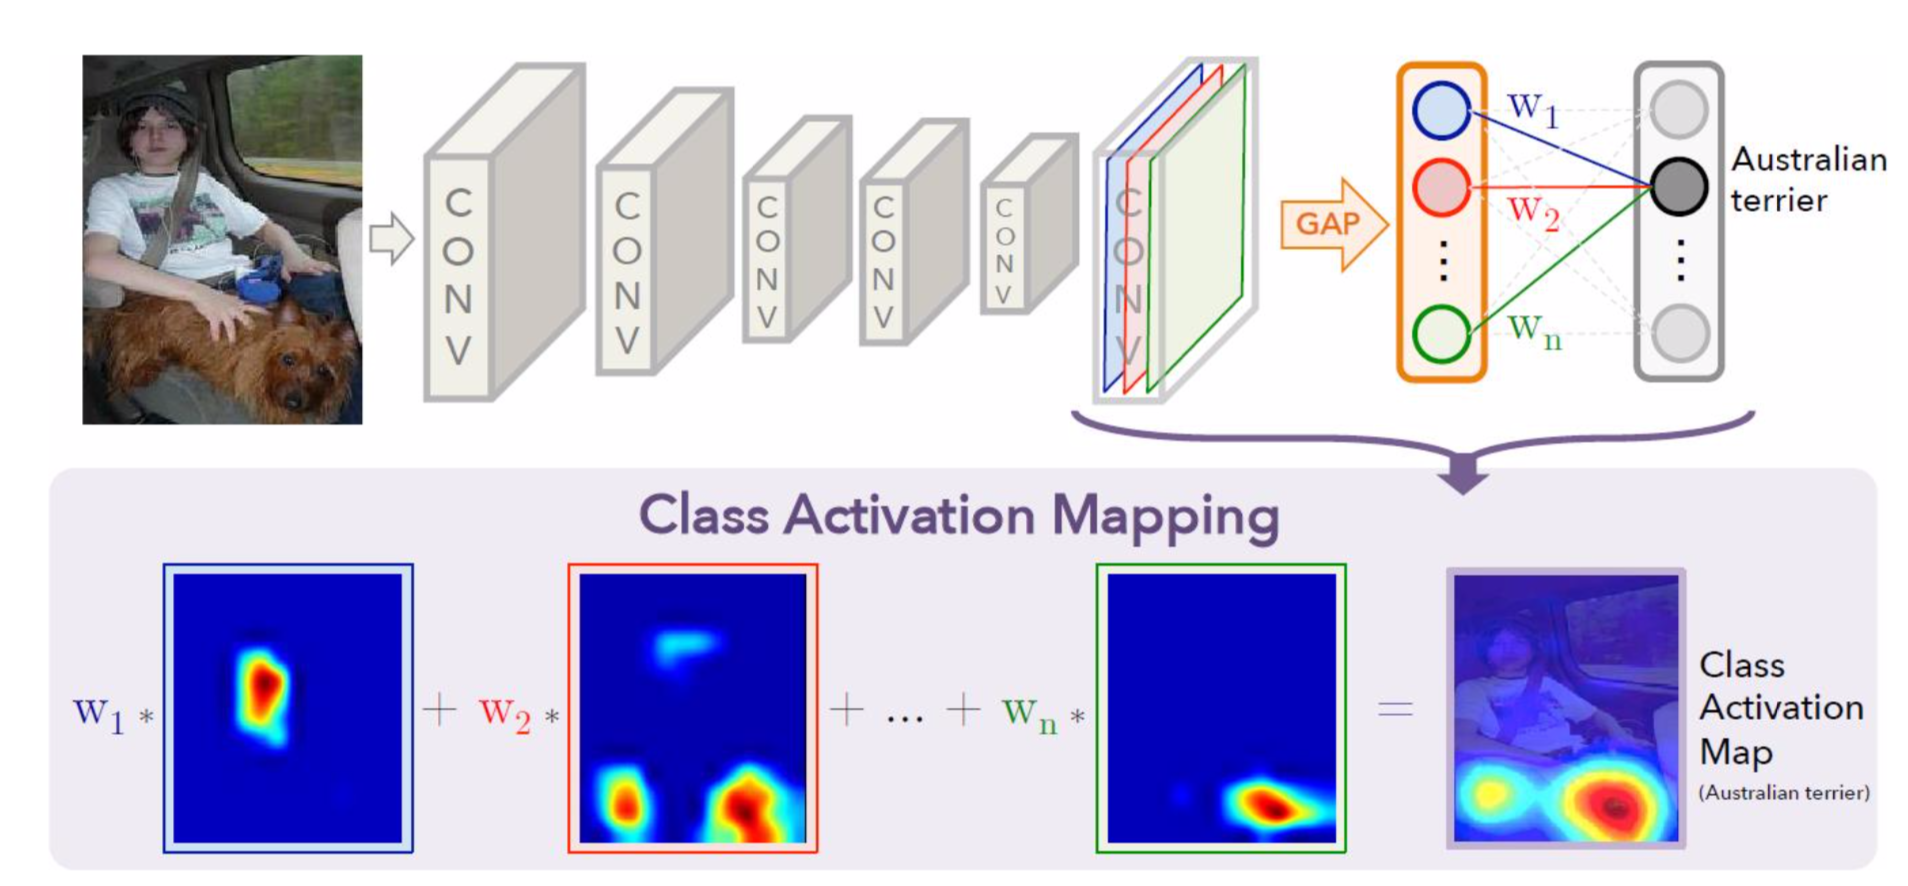
\includegraphics[width=15cm, height=6cm]{images/cam.png}
    \caption{Class Activation Map}
    \label{fig:cam}
\end{figure}
%(quando si mette una fully-connected si aumentano tantissimo i parametri quindi le performance cadono drasticamente).
\textbf{Remarks}:
\begin{itemize}
    \item[--] CAM can be included in any pre-trained network, as long as the FC layer is removed
    \item[--] The FC used for CAM is simple, few neurons and nohidden layers
    \item[--] Classification performance might drop (in VGG removing FC means loosing 90\% of  parameters)
    \item[--] CAM resolution (localization accuracy) can improve by "anticipating" GAP to larger convolutional feature maps
    \item[--] GAP: encourages the identification of the whole object, as all the part of the values in the activation map concurs to the classification 
    \item[--] \textbf{GMP} (\textbf{Global Max Pooling}): it is enough to have a high maximum, thus promotes specific discriminative features
\end{itemize}{}

The fully-connected part of the network is very simple, but it requires changing the network and loosing performance (adding a fully-connected layer drops the performance).\\ \\
\textbf{Grad-CAM} computes that weights to the gradient of back propagation, you don't even have to change the network (a fully-connected network at the end is not required) and it is good because if you get a pre-trained network for doing other stuff (captioning, object detection) you don't have to change it. You can use these heatmaps even attaching them to an existing network without the need to retrain them. 

\subsection{Object Detection}
Given a fixed set of categories and an input image which contains an unknow and varying number of instances, draw a bounding box on each object instance. A training set of annotated images with label and bounding boxes for each object is required. Each image might require a different number of outputs, depending on the number of object detected. \\ \\

In fact, the tricky part is that the number of output is not pre-defined, it depends on the input image. \\
Different solutions are proposed:

\subsubsection{Sliding Windows}
Define a certain patch (a sort of box that captures a portion of the image) size and slide this patch on the image, classify the content in that patch. If you get some output with high probability then you might take that as output of your object detection algorithm. \\
A pre-trained model is meant to process a fixed input size, so you have to slide on the image a window of that size and classify each region, assigning the predicted label to the central pixel.
There is a special class that is 'background' which means that there is no relevant object inside that patch. \\
It is very inefficient since for identify an object, e.g. a car, entirely you need a bigger bounding box. So theoretically you have to test different patch size. It does not re-use features that are "shared" among overlapping crops.  Inefficient also if you consider only a single patch size: take a patch and slide means compute convolution multiple times for each pixel because each pixel belongs to multiple patches. Moreover, each patch feeds the network independently from the others and all the operation are repeated multiple times. 
The only advantage is that there is no need of retraining the CNN.

\subsubsection{Region Proposal}
Region Proposal algorithms (and networks) are meant to identify bounding boxes that corresponds to a candidate object in the image.\\ \\
The first network performing object detection were actually based over these techniques. These algorithms have an high recall (if there is an object, those algorithms provide a bounding box), but very low precision because they provide a lots of region proposal out of a image.\\
The idea is: apply a region proposal algorithm $\rightarrow$ Classify by a CNN the image inside each proposal regions

\subsubsection{R-CNN: Region-CNN}
Object detection by means of region proposal. So given an input image, run the Region Proposal algorithm and extract a huge amount of proposals, e.g.. 2K of proposals. Modify the content of your region proposal to become a square since  the network is a standard CNN which expects a fixed input size. \\ \\
Taking the cowboy image, once extracted the regions, you squeeze the cowboy to be a square. The major drawback is that in this way you lost the proportion, relevant to understand the content. \\

 \begin{figure}[h]
    \centering
    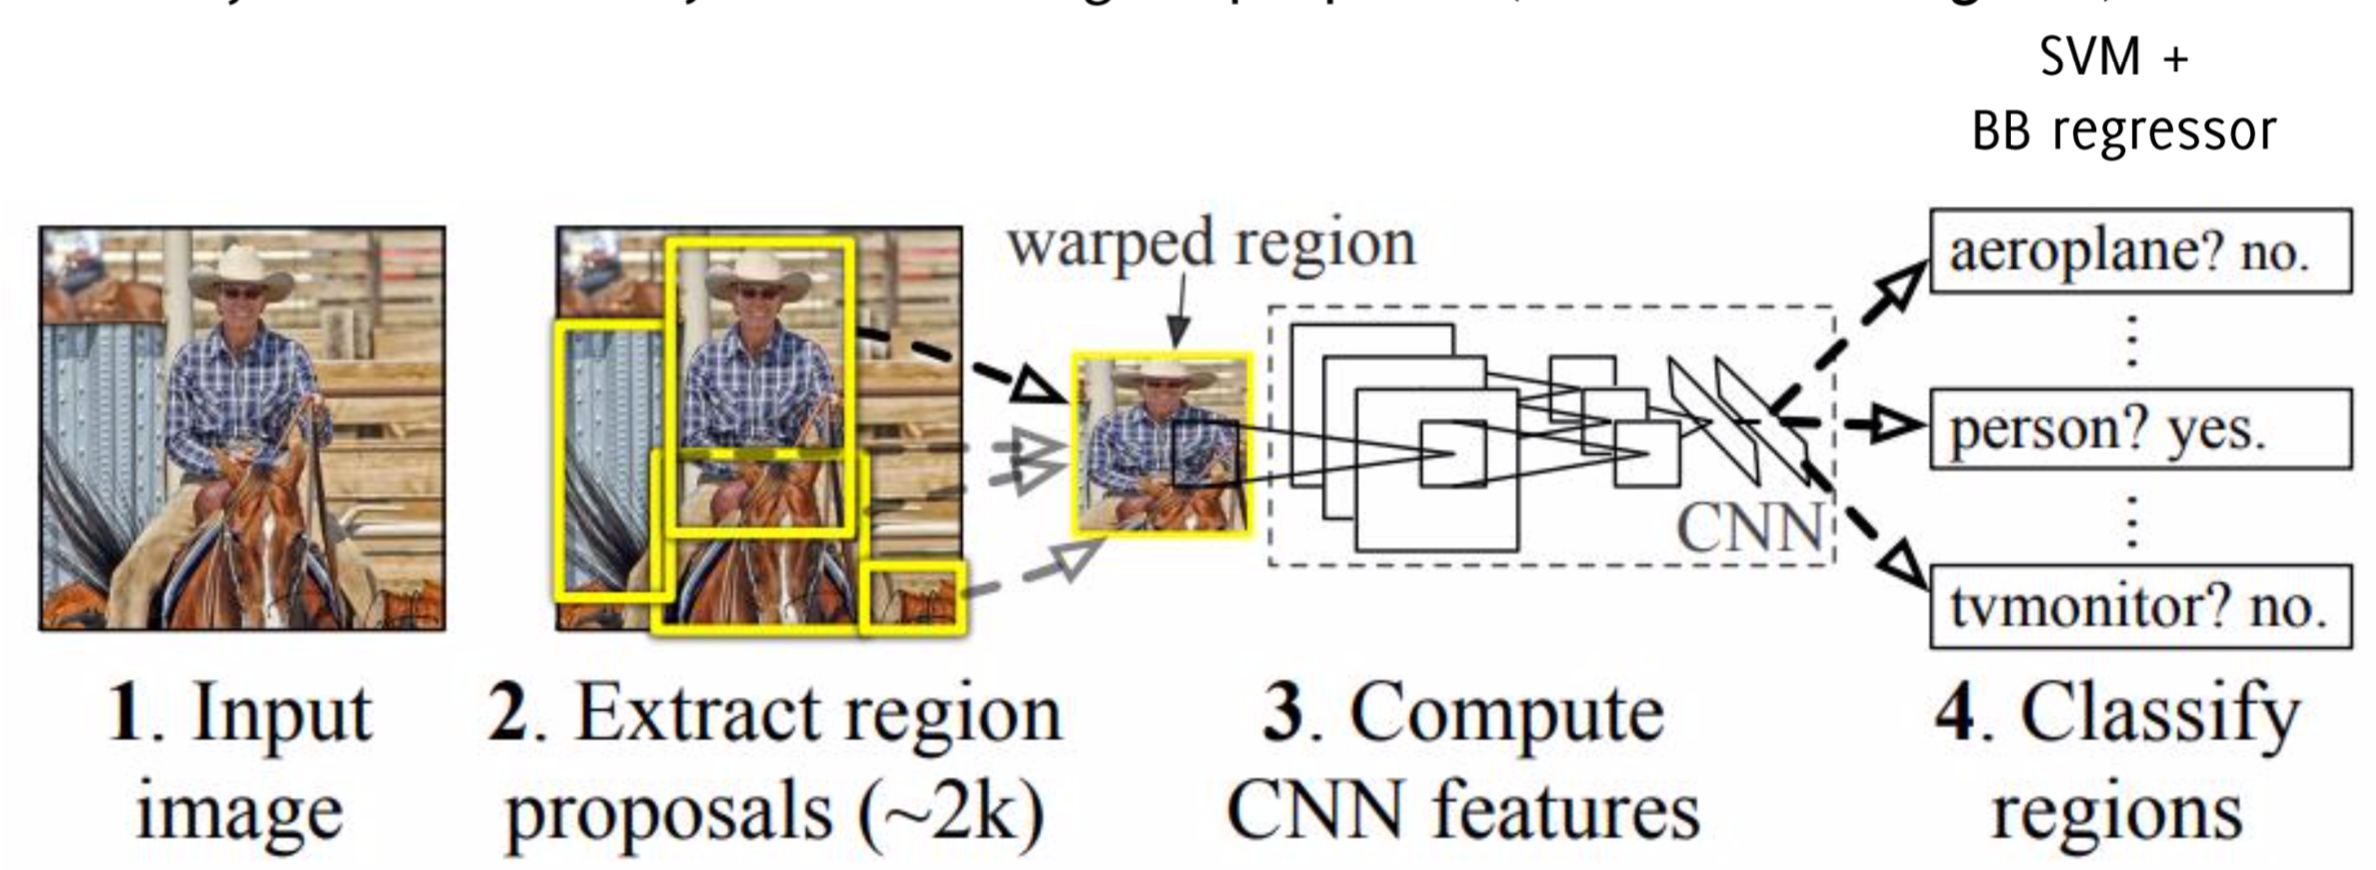
\includegraphics[width=15cm, height=6cm]{images/r_cnn.png}
    \caption{R-CNN}
    \label{fig:r-cnn}
\end{figure}

So Region Proposal detects the input, CNN extracts the features. At the end it is used a SVM in order to classify and find out what will be the label of the region proposal. On top of that, a bounding box regression in order to improve the localization, so there will be different losses. \\
There was no learning algorithm in the Region Proposal, so a very high recall. Instead, the CNN is fine-tuned during training. \\
However, this architecture has some limitations: 
\begin{itemize}
    \item[--] Ad-hoc training objectives and not an end-to-end training: fine-tune network with a softmax classifier, train post-hoc linear SVMs, train post-hoc bounding-box regressions
    \item[--] \textbf{Region proposal are from a different algorithm} (Region Proposal) and that part has not been optimized for the detection by CNN
    \item[--] Training is \textbf{slow}, you get a lot of proposal and for each of them you have to extract the features by the CNN $\rightarrow$ takes a \textbf{lot of disk space} to store features. 
    \item[--] \textbf{Inference is slow} since the CNN has to be executed on each region proposal (\textbf{no feature re-use})
\end{itemize}{}

\subsubsection{Fast R-CNN}
To save a lot of time, especially in inference time, instead of cropping the regions on the image and passing the image, cropped and resized, to another network, you can just \textbf{project the region proposals} from the input image over the last fully-convolutional layer: you have to perform all the CNN just once. 

 \begin{figure}[h]
    \centering
    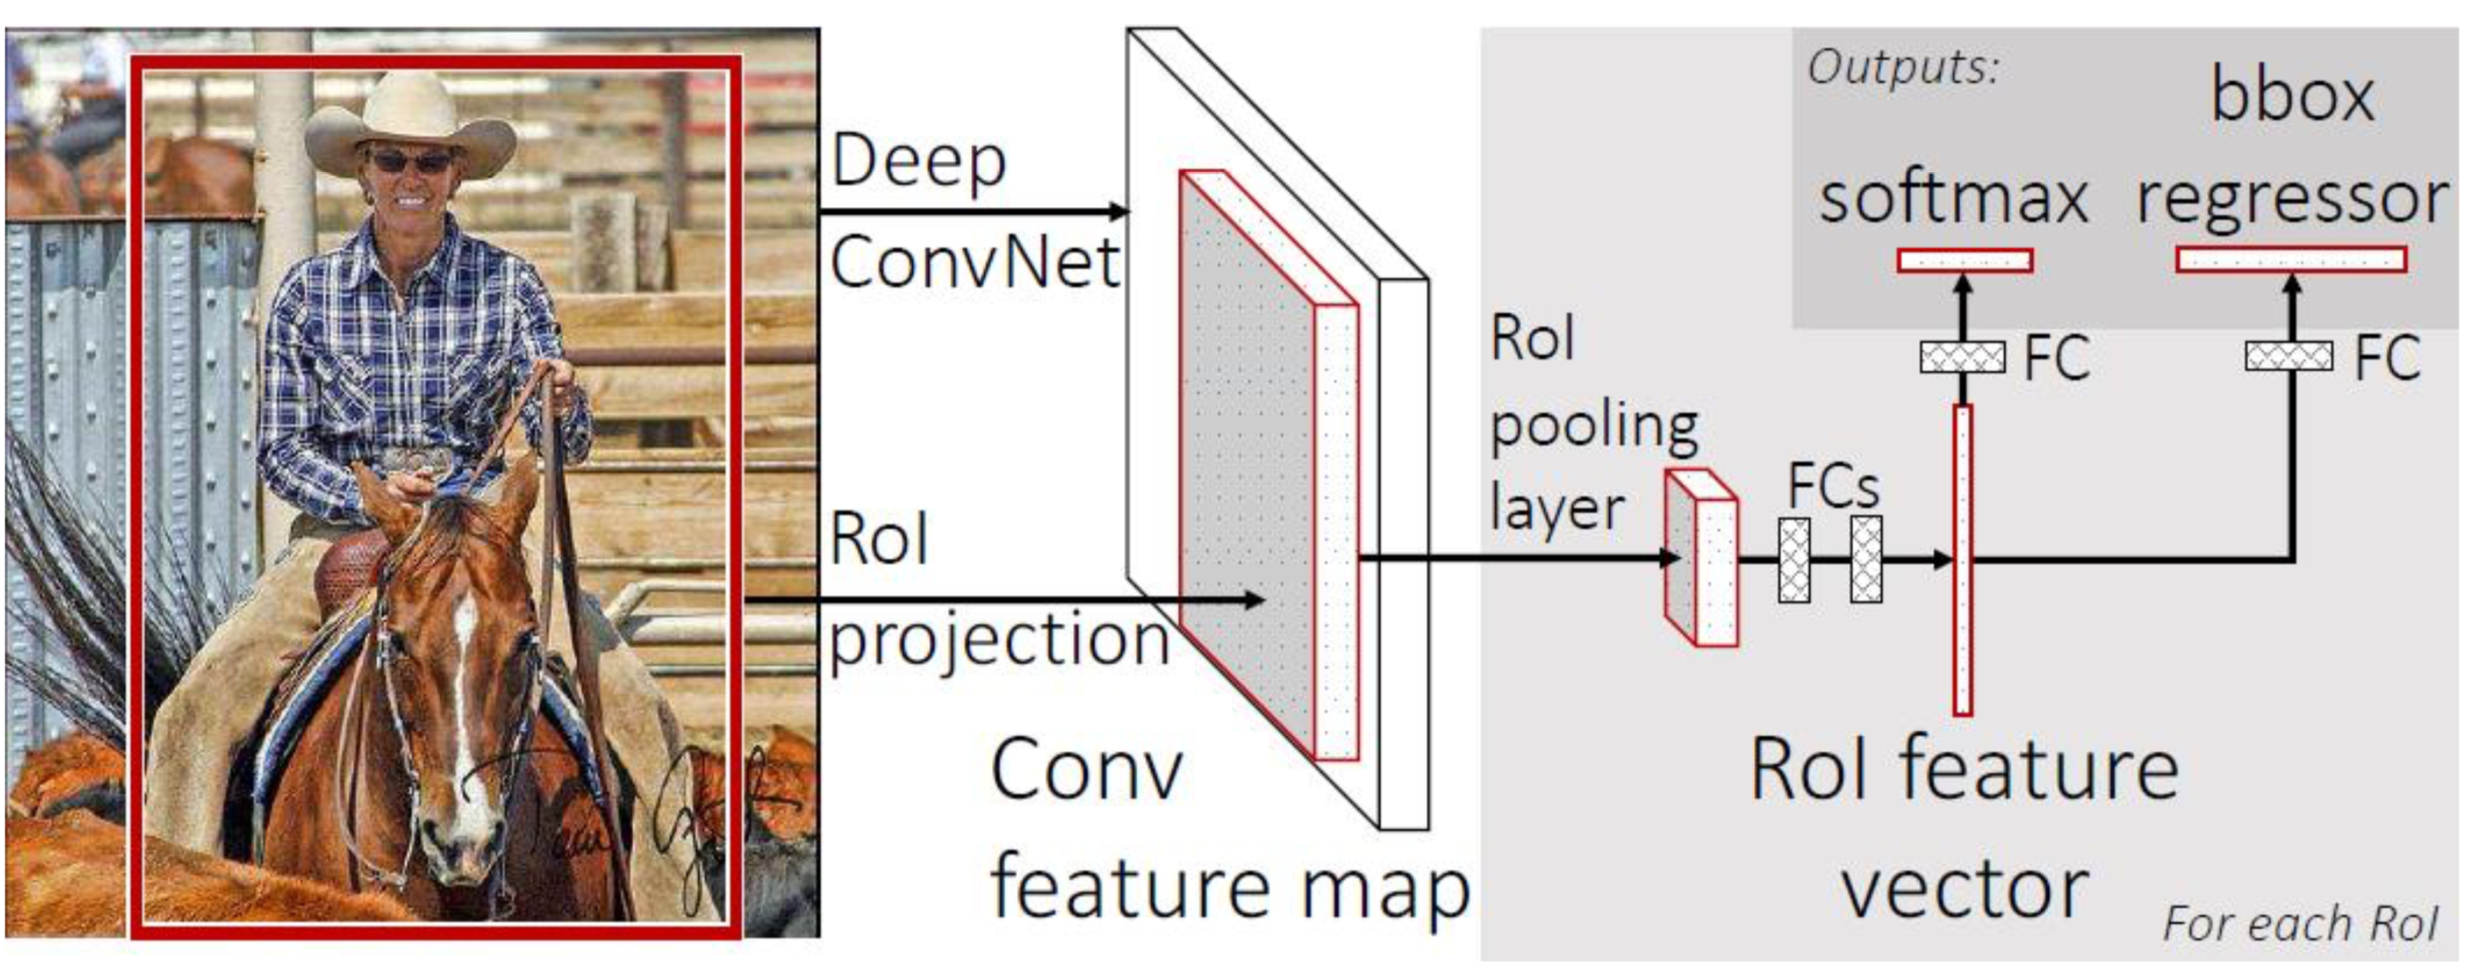
\includegraphics[width=15cm, height=6cm]{images/fast_r_cnn.png}
    \caption{Fast R-CNN}
    \label{fig:fast-r-cnn}
\end{figure}

%So you feed the image to a big CNN and the same image to a Region Proposal Algorithm. The latter returns a lot of regions, which are not used to extract a portion of the image, resized it and fed to a CNN, but you simply project this regions over the last fully-convolutional layer of the network.
%You don't have to crop and feed the same image 2000 times the same image, you have just to extract the regions and project them to the last layer. 

\begin{enumerate}
    \item The wholw image is fed to a CNN that extracts feature maps
    \item Region proposal are identified from the image and progected into the feature maps. Regions are directly cropped from the feature maps, instead from the image $\rightarrow$ re-use convolutional computation
    \item Fixed size is still required to feed data to a fully connected layer. \textbf{ROI Pooling layers} extract a feature vector of fixed size $HxW$ from each region proposal. Each ROI in the feature maps is divided in a $HxW$ grid and then max-pooling over this provides the feature vector
    \item The FC layers estimate both classes and BB location (BB regressor). A convex Combination of the two is used as a multi-task loss to be optimized (as in R-CNN, but no SVM here)
    \item Training in an end-to-end manner
\end{enumerate}{}

Some issues: here you are using this network only to extract features; once you have these feature and you have to feed an architecture with them for classification, you have to fix the  input size. So the problem has been postponed: what Ross (the creator of Fast R-CNN) does is \textit{ROI Pooling layer}: whatever partial size the projected region proposal has, you divide it in $HxW$ blocks and you perform max pooling on these regions. \\
What you get is a volume with a fixed special extent: it's like max pooling which works on larger neighbours if the regions are larger, and smaller vice-versa. \\
Still the cowboy is squeezed but it is \textit{squeezed on the features} and with the max pooling. Then you can predict the class and the bounding box location (softmax and BBox regressor). \\ \\

By doing this you can \textit{backpropagate this loss through the whole network}, which becomes incredibly faster than R-CNN during testing. Now that convolutionss are not repeated on overlapping areas, the vast majority of test is spent on ROI extraction: most of inference time is spending on extracting Region Proposal.

\subsubsection{Faster R-CNN}
Faster R-CNN gets close to real-time object detection. You move Region Proposal inside the network: you train a network in order to extract the convolutional features, from them you extract a region proposal. You do not look at the image anymore, you look at the feature map directly. \\ 

Instead of the ROI extraction algorithm, a region proposal network (\textbf{RPN}) is used in order to extract a region proposal from the convolutional features. So RPN operates on feature maps of the last convolutional layers. The remaining operation are very similar to a Fast R-CNN \\ 

You feed your CNN with an input image, you get a volume (the convolutional features) and there you run RPN. \\ 
The Region Proposal network works as follows: it takes a filter of $3x3$ and slide the feature maps. It maps (by 1x1 convolution) the region to a lower dimension vector. In each point it consider $k$ anchor boxes, i.e. different ROI size/proportions (k-possible templates for region), thus there  $HxWxk$ candidate anchors.\\
The classification network (\textit{cls} network) is trained to predict the object probability, i.e. that each anchor contains an object \textit{[obj, no-obj]} $\rightarrow$ $2k$ probability estimates.  
The region network (\textit{reg} network) is trained to adjust the anchor to the object ground truth $\rightarrow$ $4k$ estimates.\\
There is no need to design different RPN to account for the $k$ different anchors. \textbf{Anchors just influence the way labels of RPN are comuted}. \\
Training now involves 4 losses: RPN classify object/non-object, RPN regression coordinates, final classification score, final BB coordinates. During the training, object/non-object ground truth is defined by measuring the overlap with annotated BB. \\
The network becomes much faster also because you don't have to design a different network for each shape of region proposal, you just train the network to predict for each of these $k$ different outputs, which correspond to an object in the image. \\
At test time:
\begin{itemize}
    \item Take the top ~300 anchors according to their object scores
    \item Consider the refined boundig box location of these 300 anchors
    \item These are the ROI to be fed to a Fast R-CNN (ROI pooling to perform the downsampling)
    \item Classify ROI
\end{itemize}{}
Therefore, Faster R-CNN provides to each image a set of BB with their objectness score.\\
It's still a \textbf{two stage detector}, where in the first stage:
\begin{itemize}
    \item run a backbone network (e.g. VGG16) to extract features
    \item run the Region Proposal network to estimate circa 300 ROI
\end{itemize}{}

In the second stage (the same as in Fast R-CNN):
\begin{itemize}
    \item Crop features through ROI pooling (with alignment)
    \item Predict object class using FC + softmax
    \item Predict bounding box offset to improve localization using FC + softmax
\end{itemize}{}
%for each location, where $HxWxk$ is the special extent of this volume, you consider 3x3 regions in the feature map, so 3x3xN. It performs a one-by-one convolution to reduce the size of the image. So you get a vector reduced representation of 256-dimension and out of this vector you perform a regression over different location in order to determine where there is a region there. So in particular you have k-possible templates for region. For each pixel, you take a subvolume, you map it in a 256-dimensional vector and you have a prediction where this is the location of k different region proposal which are of different proportion. So you train your network to predict HxWxk possible shapes for the region proposal. You don't have to design a different network for each shape of region proposal, you just train the network to predict for each of these k different outputs, which correspond to an object in the image.
%So the network is predicting whether in each point in the feature map there is one of those k possible bounding boxing. 
%To train it, you need 4 different losses: 1 classify the object, 1 for the regression of the coordinates, 1 to classify the final classification score and the final bounding box score. 
%This allows you to take at test time 300 most probable bounding boxes (anchor points), then consider only these 300 as candidate location for an output and once you have them, you feed them to the first network. The rest is the same: ROI pooling to perform the down sampling and then you classify them. 
%It is a two stage detector. 
%This provides an incredible speed-up. 

\subsubsection{You Only Look Once (YOLO)/ Single Shot Detectors (SSD)}
R-CNN methods are based on Region proposal, but there are also region-free methods, like YOLO or SSD. Detection networks are indeed a pipeline of multiple steps. In particular, region-based methods make it necessary to have two steps during inference. This can be slow to run and hard to optimize, because each individual component must be trained separately.\\ \\
In YOLO 
\begin{quote}
    \textit{We reframe the object detectino as a single regression problem, straight from image pixels to bounding box coordinates and class probabilities}
\end{quote}{}
And solve these regression problems \textbf{all at once}, with a large CNN. \\
These algorithms don't have to go to this two stage phases, they cast all the object detection as bounding box regression problem, starting from the image. \\

In YOLO: 
\begin{enumerate}
    \item Divide the image in a coarse grid
    \item each grid cell contains $B$ \textit{base-bounding boxes} associated
    \item For each cell and \textit{base-bounding box} we want to predict: 
    \begin{itemize}
        \item the offset of the base bounding box, to better match the object: (dx, dy, dh, dw, objectness score)
        \item The classification score of the base-bounding box over the $C$ considered categories (including background)
    \end{itemize}{}
\end{enumerate}{}

The whole prediction is performed in a single forward pass over the image, by a single convolutional network. Training this network is sort of tricky to assess the loss (matched/not-matched).\\
YOLO/SSD shres a similar ground of the RPN used in Faster R-CNN. Typically networks based on region-proposal are more accurate, single shot detectors are faster but less accurate.
%you crop the image on a grid; inside of each it propose a anchor, so a candidate location for a possible region proposal and then train a network which is meant to determine whether each of this region can be the location for an object and the corresponding bouding box. 
%This part is sort of similar as the Faster-R-CNN. This is like one-shot. 
